\pagebreak

\subsubsection*{Magnetometer}
Magnetometers are used to detect large bodies of metal. This can be a useful application for the detection of parked vehicles in parking spaces. As illustrated in this paper \citep{Villanueva2016CrowdsensingMonitoring}, tests are carried out with the magnetometer on a Samsung Galaxy S4. The study was conducted in three different scenarios. In the first scenario, the goal was to try and classify different magnetometer readings in various situations. Additionally, an investigation into whether an active engine interferes with the magnetometer readings. The combinations investigated in the study are as follows:

\begin{itemize}
    \item (ssb) Test vehicle engine stopped, test vehicle stopped, adjacent vehicles on both side of test vehicle
    \item (rsb) Test vehicle engine running, test vehicle stopped, adjacent vehicles on both sides of test vehicle
    \item (rsl) Test vehicle engine running, test vehicle stopped, vehicle on left side of test vehicle
    \item (rsn) Test vehicle engine running, test vehicle stopped, no vehicles close to test vehicle
    \item (ssn) Test vehicle engine stopped, test vehicle stopped, no vehicles close to test vehicle
    \item (ssl) Test vehicle engine stopped, test vehicle stopped, vehicle on the left side of test vehicle
\end{itemize}

The study successfully classifies readings through the use of \ac{SVM}. \ac{SVM} is a supervised machine learning algorithm. \ac{SVM} is generally used for classifications and regression \citep{Suykens1999LeastClassifiers}. 

Through the use of \ac{SVM}, the readings from the magnetometer can be classified. For the purpose of illustration, figure \ref{figure:magnetometer} shows the magnetometer readings obtained by the study.

With these classifications, the mobile phone that performed the information sensing could relay this information to a central server. In this way, the central server will have additional knowledge regarding parking space occupancies within that specific phones' area.

\begin{figure}[H]
    \centering
    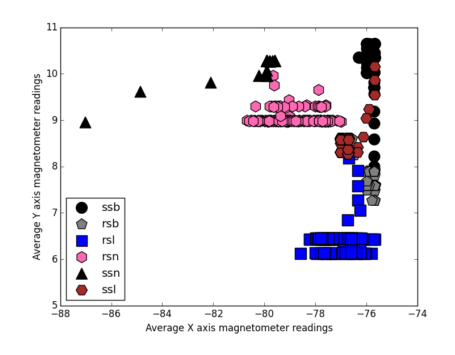
\includegraphics[width=0.75\linewidth]{./Images/MAGNETOMETER.PNG}
    \caption{Magnetometer Readings}
    \label{figure:magnetometer}
\end{figure}

In the second scenario, the aim was to investigate whether a moving test vehicle equipped with a mobile magnetometer is able to detect vacant parking spaces. The setup to this scenario includes a line of parked vehicles with one vacant spot. The test vehicle drives alongside the line of parked vehicles, emulating a vehicle driving down a street of parked vehicles. The magnetometer showed a significant reading as it passed the vacant spot, thus the investigation concludes that it is successful in detecting vacant parking spots while the test vehicle is moving.

In the third scenario, the distance of a parked vehicle to the test vehicle is investigated. The test begins with the test vehicle parked beside another vehicle. The test vehicle is then moved further and further away from a parked vehicle. The results show that the magnetometer readings are useless unless vehicles are very near.

The results obtained through this paper shows that it is possible to use magnetometers to detect parking space occupancies. However a suitable application has yet to be discussed. A magnetometer may only sense parking spaces when the device is relatively near. Unless this is incorporated into a crowdsensing scheme, there is no incentive for drivers to cruise a parking lot or urban streets sensing spaces for other drivers. Integration of magnetometers onto taxis, as previously discussed in the laser range finder section, could also be considered. By attaching magnetometers to public transport or taxis, they may be able to scan parking areas for parking space availabilities.